\newpage

\section{Classification}
\subsection{Deep neural networks}
	Deep Learning technologies based on convolutionnal neural networks are revolutionising the field of image classification. In 2012, during the ImageNet Large Scale Visual Recognition Challenge, the algorithm submitted by Alex Krizhevsky, wich is a neural network architecture called AlexNet, outperformed the everyother algorithms. Since, numerous other architecture have been deisgned, and deep neural network have climb a new step in Image recognition.
\subsubsection{Layers}
	Neural networks are a combination of differents layers from wich data flows threw. Layers are combination of some elementary operations. There is a few different types of neural network layers :
	\begin{itemize}
		\item Dense layers : 
		\item Convolutionnal layers : One filter (=kernel) is applied in a convolutional way by translating the kernel on all the surface of the image. This way, numerous filters can be applied at one step of an image, creating differents set of new features. Advantages : sparse interactions , parameter sharing and equivariant representa-
		tions
		\item Pooling layers : Pooling layers reduce dimensions, and increase translation small invariance. On a set of locally near pixels, it "replace the output of the net at a certain location with a summary statistic of the nearby output". the information (in different ways : taking the max, the min, the mean...)
		\item Other layers : ???
	\end{itemize}
\subsubsection{Regularization}
	Drop out...
\subsubsection{Learning parameters}
	Batch size, epochs, steps per epochs... 
\subsection{AlexNet}
AlexNet is a convolutional architecture designed by Alex Krizhevsky[]. It is based on 5 convolutionnal layers followed by 3 denses layers.
\begin{figure}
   	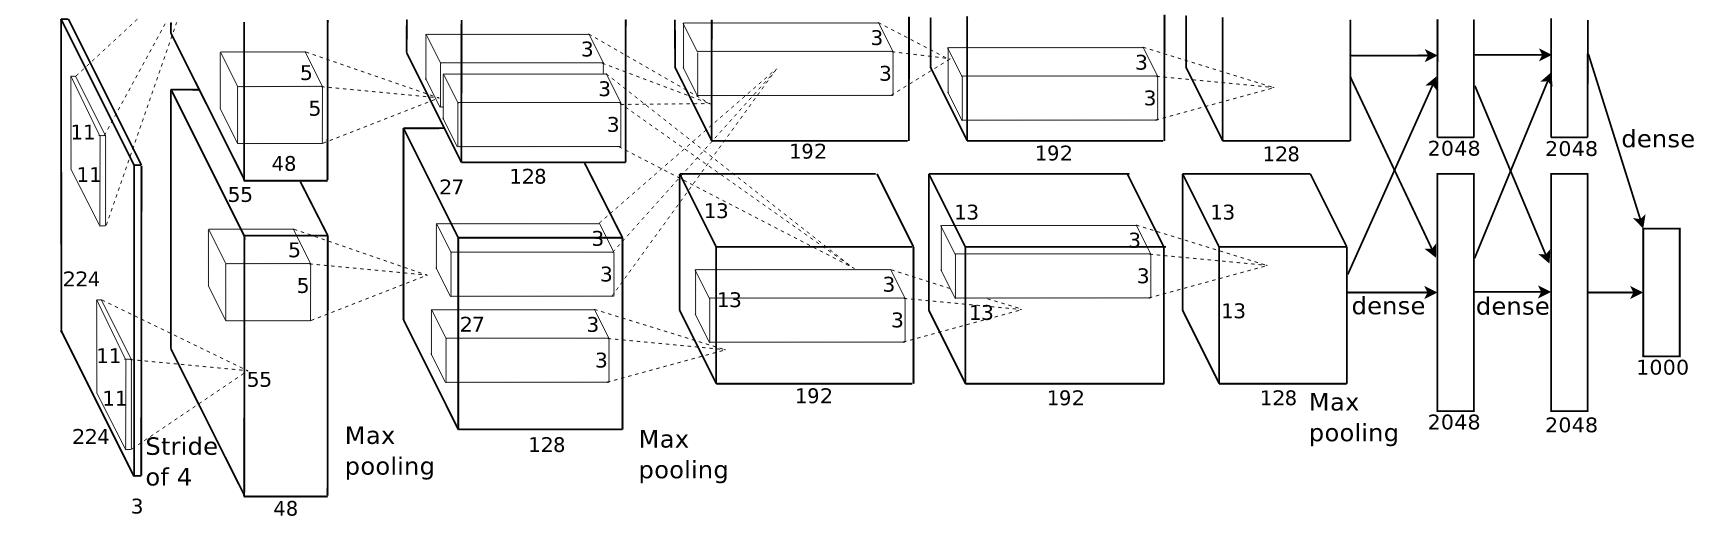
\includegraphics[scale = 0.2]{images/alexnet_architecture.png}
\end{figure}

The weights of the network trained on the ImageNet database are available online. Therefore, we can directly evaluate our test data without training. The original number of outputs is 1000.Image input dimensions need to be 227*227. We can't change it without loosing the training weights on the Dense layers.\\
On the figure, all the layers are splitted in two parts. This way, the network can be trained on 2 differents GPU. It doesn't change how the network behave, since there is a merging after each layer. \\
The "recognizing image style" paper uses the notation DecafX, corresponding to the features outputs of the Xth layer. The term decaf comes from the framework used, Caffe[source]. They have reached to the conclusion that classifying the output features of the sixth layer (decaf6) can lead to good results. So we took the output of the 6th layer, on wich we added a dense layer that we trained in order to have 25 outputs. We did the same operation with the features of the fifth output d(Decaf5) in order to verify that the 6th layer is really the best one.\\


\subsection{Other nets ?}


\subsection{Results}
	\textbf{RESULTS :}\\
	0.356 accuracy percentage was expected. We obtained 0.367 on the all validation set, and 0,370 on the all test set (batch size: 256, epoch 32 with an horizontal flip. 8h34 on GTX 1080Ti )\\
	
	\begin{figure}[ht]
		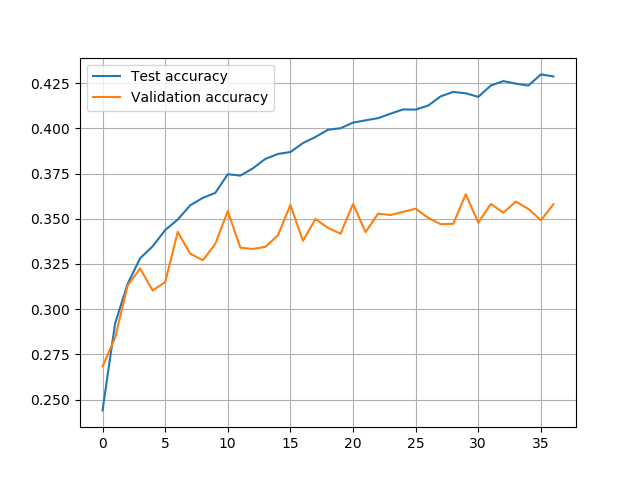
\includegraphics[scale = 0.8]{images/results_decaf6.png}
		\caption{Train and validation accuracy with decaf6 features}
	\end{figure}
	
	With the 5th layer features, the results were 0,323 max, and seemed to overfitt at the end.\\

\begin{figure}[ht]
	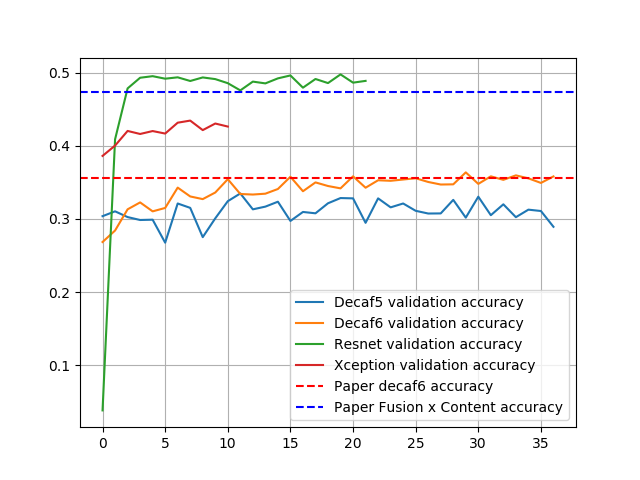
\includegraphics[scale = 0.8]{images/general_results.png}
	\caption{Validation accuracy on different networks}
\end{figure}


	
\begin{tabularx}{10cm}{|X|c|c|}
	 \hline
	 \textbf{Classifier} & \textbf{Top-1 accuracy} & \textbf{Top-5 accuracy}  \\
	 \hline
	 Alexnet(Decaf5) & 0.334 & 0.749\\
	 \hline
	 Alexnet(Decaf6) & 0.370 & 0.769 \\
	 \hline
	 Inception &  & \\
	 \hline
	 Xception & 0.422 & 0.830\\
	 \hline
	 Resnet & \textbf{0.495} & 0.878\\
	 \hline
	 \textbf{Decaf6 from Paper} & 0.356 & \\
	 \hline
	 \textbf{"Fusion x Content" from Paper} & 0.473 & \\
	 \hline
\end{tabularx} 


\subsubsection{Critics}
	The paper seems to obtain his accuracy by averaging all the accuracies between the classes.



